\documentclass[a4paper]{article}
\usepackage[a4paper,pdftex]{geometry}
\usepackage[english]{babel}
\usepackage{amsmath,amsfonts}
\usepackage[pdftex]{graphicx}
\usepackage{epstopdf}
\usepackage{fancyhdr}
\usepackage{lastpage}
\usepackage{setspace}
\usepackage{xcolor}
\usepackage{hyperref}
\usepackage{url}
\usepackage[toc,page]{appendix}
\usepackage[T1]{fontenc}   

% Page margins
%\setlength{\oddsidemargin}{5mm}
%\setlength{\evensidemargin}{5mm}

% Page style
\pagestyle{fancy}

% Page numbering
\lhead{Sensor Fusion on a mini Unmanned Vehicles}
\cfoot{}
\rfoot{\thepage}

% TITLE FORMAT
\newcommand{\HRule}[1]{\rule{\linewidth}{#1}}
% BIBLIOGRAPHY

\makeatletter
\def\printtitle{
    {\centering \@title\par}}
\makeatother                  

\makeatletter
\def\printauthor{
    {\centering \large \@author}}
\makeatother

% TITLE
\title{
\HRule{0.5pt} \\
\LARGE \textbf{\textsc{Sensor Fusion on a mini Unmanned Vehicle}}\\[0.5cm]
\normalsize \textsc{Integrating vision-based algorithms on an Parrot AR.Drone to autonomously follow linear shaped structures in a landscape.}
\HRule{2pt}\\ [0.5cm]
Camiel R. Verschoor\\
10017321\\
\vspace{1cm}
Bachelor thesis\\
Credits: 18 EC\\
\vspace{0.5cm}
Bachelor Opleiding Kunstmatige Intelligentie\\
\vspace{0.25cm}
University of Amsterdam\\
Faculty of Science\\
Science Park 904\\
1098 XH Amsterdam\\
}

% AUTHOR
\author{\normalsize
\emph{Supervisors}\\
Dr. A. Visser\\
\vspace{0.25cm}
Informatics Institute\\
Faculty of Science\\
University of Amsterdam\\
Science Park 904\\
1098 XH  Amsterdam\\
\vspace{0.5cm}
Drs. G. Poppinga\\
\vspace{0.25cm}
Defense Systems\\
Aerospace Systems\\
National Aerospace Lab\\
Anthony Fokkerweg 2\\
1059 CM Amsterdam\\
\vspace{1cm}
July 24th, 2012\\
}

% BEGIN DOCUMENT
\begin{document}

% TITLE PAGES
\thispagestyle{empty}
\begin{center}
\Large\textsc{Sensor Fusion on a mini Unmanned Vehicle}\\
\normalsize\textsc{Integrating vision-based algorithms on an Parrot AR.Drone to autonomously follow linear shaped structures in a landscape.}

\vspace{2cm}

\begin{figure*}[!ht]
\centering
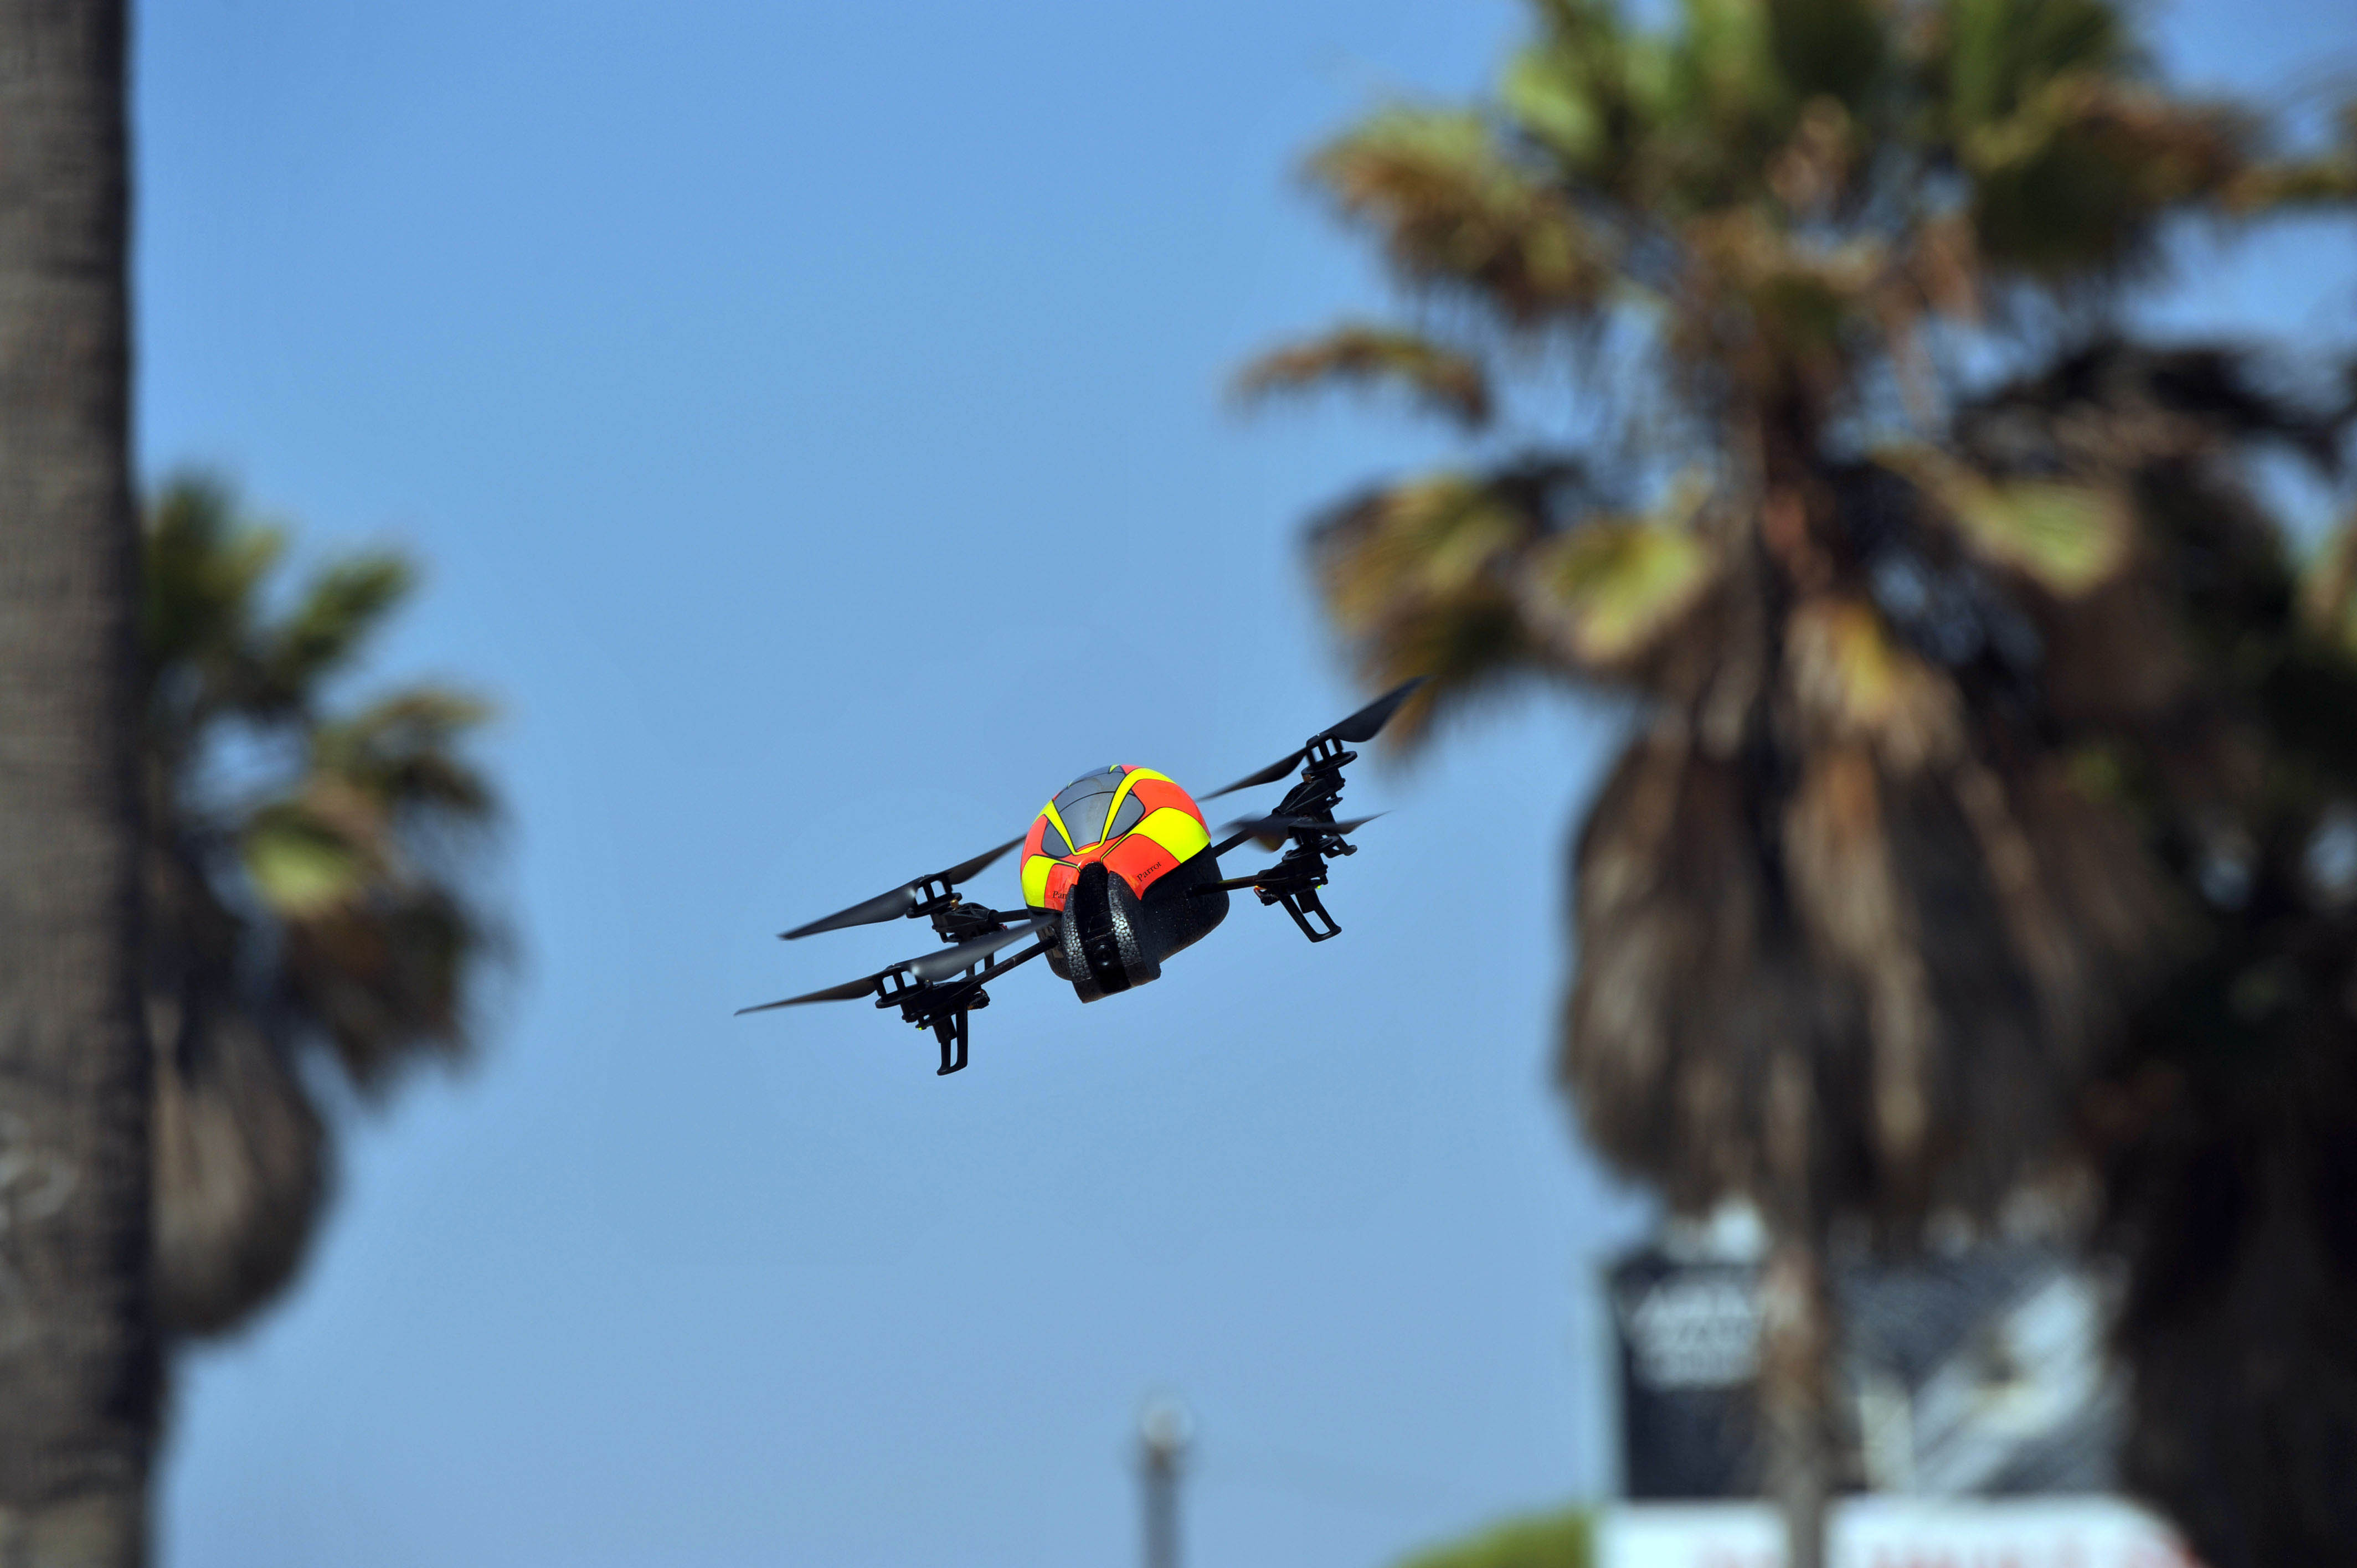
\includegraphics[width=\textwidth]{images/title.jpg}
Photo by: \href{http://ardrone.parrot.com/album/}{Parrot SA}
\end{figure*}

\subsubsection*{A Bachelor Thesis by Camiel R. Verschoor}
\end{center}
\newpage

% EMPTY PAGE
\thispagestyle{empty}
\mbox{}
\newpage

% THESIS INFORMATION
\thispagestyle{empty}
\printtitle
\vfill          
\printauthor
\newpage

% ABSTRACT
\thispagestyle{empty}
\section*{Abstract}
To be written.
\section*{Acknowledgements}
I would like to thank my supervisors Arnoud Visser and Gerald Poppinga for their support and guidance. Furthermore, I am grateful to Nick Dijkshoorn for the distribution of his development framework, AR.Drone SLAM, and his support installing it. I also like to thank Robrecht Jurriaans for borrowing his AR.Drone. Likewise, I would like to thank Rob van Holstein for the construction of a 3D model of the frame that is holing the mirror. Moreover, I like to thank Christian Muller for helping collecting the dataset and learning me to fly a quadcopter manually. Furthermore, I am grateful to the National Aerospace Lab for the internship and the visit to the International Micro Aerial Vehicle Conference and Competitions. Lastly, I am thankful to my girlfriend and my family for their support and encouragement.
\newpage

% TABLE OF CONTENTS
%\thispagestyle{empty}
\tableofcontents
\newpage
\setcounter{page}{1}
% SPACING
\onehalfspace

% INTRODUCTION
\section{Introduction}
In robotics one of the main goals is to develop mobile robots that can operate autonomously in the real world environment. These autonomous robots have various purposes and are used for a wide range of applications such as inspection, exploration and rescue. In rescue, robots are expected to operate in dangerous environments without putting human lives at risk for example, during disasters or life rescue operations. Even though reasonable developments have been made in the robotics field, robots cannot operate autonomously in the real world yet.

One of the main requirements of an autonomous robot is the ability to navigation in the operational environment. The traditional approach to navigate through the outdoor environment is via pre-planned paths based on a Global Positioning System (GPS). The main shortcoming of GPS is that it cannot be used in every environment as it needs to receive data signals from at least four different satellites \cite{Bajaj2002}. Inside buildings and in several outdoor areas GPS is not convenient for navigation. In urban areas GPS is found to be especially unreliable. In order to navigate through these environments other sensors and navigation techniques need to be applied. Since there are several linear structures in the environment such as rivers, roads and power lines, line-following is one possible approach to navigate through an environment. Line-following is a classic technique in robotics as it has been successfully used for ground robots numerous times \cite{Sampei1995, Dupuis2006}. For other robots and sensor configurations, open problems still remain. One of these is navigation for micro aerial vehicles (MAVs), which have a limited sensor composition due to their limited payload. For MAVs line-following is a greater challenge due to the extra dimension it can move in comparing to the average ground robot. Where the sensors of a ground robot can rely on the stability of the ground, while the sensors of a MAV have to count on the stability of the platform during a flight. Therefore, MAV are more likely to measure noisy data, which interpreting algorithms should resist.

\begin{figure}[!ht]
	\centering
	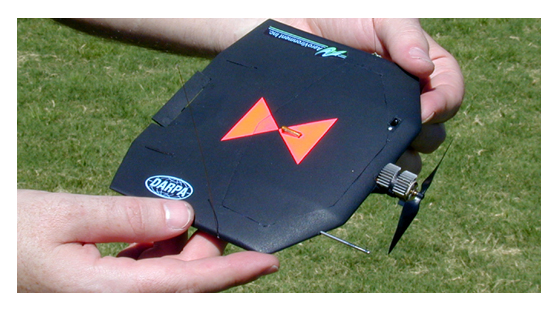
\includegraphics[width=0.5\textwidth]{images/blackwidow.eps}
	\caption{The Black Widow \cite{Grasmeyer2001} was the first operating micro aerial vehicle system, a development which was finalized in 1999 by AeroVironment for Defense Advanced Research Projects Agency (DARPA). The Black Widow can fly for up to 20 minutes and carries a very small color video camera.}
	\label{blackwidow}
\end{figure}

A micro aerial vehicle (MAV) is a subclass of the Unmanned Aerial Vehicles. Due to their small size, the MAV can operate in numerous robotic applications, for instance, search \&  rescue, inspection and exploration. AeroVironment Black Widow\cite{Grasmeyer2001} (figure \ref{blackwidow}) is the first MAV operating in the field. Another type of MAV is the quadcopter, which is controlled by four rotors. Quadcopters provide manoeuvrability and stability, which is suitable for indoor and urban flights. As a result of recent developments, small quadcopters with on-board stabilization can be purchased conveniently. Due to this, the research regarding this platform is moving towards intelligent applications, which demand information of the surrounding environment. Nevertheless, the fast movements and the limited amount of sensor combination mean that it is still a challenge to develop navigation methods for these platforms.

\subsection{International Micro Aerial Vehicle Conference and Competitions}
The International Micro Aerial Vehicle (IMAV)\footnote{\url{http://www.imav2012.org/}} conference and competitions is an initiative that attempts to share and demonstrate new MAV technology. The competitions emphasizes on flight dynamics and autonomous flight. The IMAV consists of an indoor and outdoor competition, where these aspects are extensively tested in the various challenges. The high level of autonomy is stimulated in this competition as the rules give significantly more points to teams that operate autonomous flights. One of the problems participants have to solve is autonomous navigation through the environment. Although teams are allowed to used visual aids (ie. markers) problems in this area remain. The possible contribution of this thesis to the IMAV competition is a vision-based navigation technique for following linear-shaped objects. This navigation technique can aid autonomous flights during the challenges of the IMAV.

\subsection{Platform and Framework}
The Parrot AR.Drone (figure \ref{ardrone}) is a wireless controlled flying quadcopter built by the French company Parrot SA\footnote{\url{http://www.parrot.com}}. The quadcopter is made of plastic and foam and is about 30 centimetres long. It carries a horizontal and a vertical camera opening the door for the development of various visual applications. The inertial measurement unit in combination with optical flow and a ultrasound sensor provide on-board stabilization during flights allowing the quadcopter to hover in the same place. 

\begin{figure}[!ht]
	\centering
	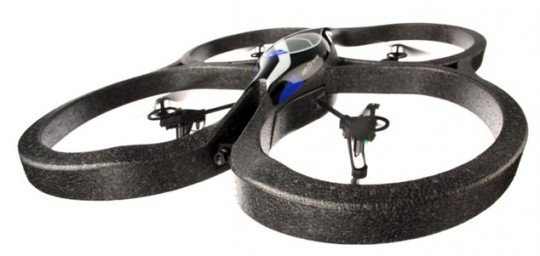
\includegraphics[width=0.5\textwidth]{images/ardrone.jpg}
	\caption{The Parrot AR.Drone is equipped with two cameras and several inertial sensors. The development is driven by commercial, government, research and military purposes. The small quadrotor allows remote observation of hazardous environments inaccessible for humans and ground robots.}
	\label{ardrone}
\end{figure}

AR.Drone SLAM \cite{Dijkshoorn2012} is a development framework for the Parrot AR.Drone, a quadcopter, developed and proposed by N. Dijkshoorn. This framework contains a real-time Simultaneous Localization and Mapping (SLAM) implementation based on a down-pointing camera. Therefore, it allows a MAV to know its position and movement in the environment by generating a feature map of the environment so the MAV can localize itself on this map. Furthermore, the framework contains a 3D mouse controller, a keyboard controller, a visual map and an elevation map. Due to the framework the robot acquires more information of the environment compared to the software of the manufacturer. This information can aid the robot in navigation. In chapter \ref{platform} and \ref{framework} the platform and framework will be explained.

\subsection{Research questions and objectives}
In robotics one goal is to develop mobile robots that can advance robustly and truly autonomously in real world situations. One of the main requirements is the ability to navigate autonomously. Since there is no sufficient GPS signal available in urban and indoor environment, robots need to rely on other sensors.

Line-following is proven to be a simple navigation task for ground robots. However, this navigation task is not implemented yet on unmanned aerial vehicles. Since there are various linear structures in the environment, line-following should be a suitable navigation technique.

Therefore, the main research question is to find a robust vision-based approach to autonomously navigate over linear shaped structures. This main research question is divided up in the following sub-questions:
\begin{itemize}
\item What is the optimal configuration for the optical sensors of the platform to follow a line?
\item What edge and motion detector algorithms are suitable to detect and track a line in a indoor environment?
	\begin{itemize}
	\item Which algorithms should be tested?
	\item Which algorithms should be used?
	\end{itemize}
\item What is the performance and robustness of different vision-based methods to navigation over a linear structure in a indoor environment?
\end{itemize}
In order to perform line-following navigation, first, a line should be detected. Secondly, the angle between the quadrotor and the line is calculated. Finally, the quadrotor adjusts its movements in order to navigate over the line. These steps are repeated until the end of the line has been reached.

% TODO: BETER
\subsection{Outline}
Chapter two gives an overview of the the theory this thesis relies on. First, the Computer Vision algorithms this thesis is based on are explained and then the navigation techniques will be discussed. Chapter three gives an overview is given over the related research regarding line-following on unmanned aerial vehicles. The robotic platform, Parrot AR.Drone, is discussed in chapter four. The construction of the platform is explained, the hardware it contains will be listed and the software development kit will be addressed. Chapter five will give an overview of the framework AR.Drone SLAM. The main architecture and functionalities will be briefly discussed. In chapter six the experiments are illustrated and in chapter seven the results will be presented. Chapter eight will discuss the results found in the experiments and elaborate on them. Finally, in chapter nine the conclusion of this thesis will be presented and directions for future research will be proposed.

\newpage
\section{Theory: Vision and Navigation}
In this chapter, the basics of the theory this thesis relies on is explained. The work presented in this thesis is based on previous research regarding vision-based algorithms on the AR.Drone \cite{Jurriaans2011} and the Open Source Computer Library (OpenCV) \cite{Bradski2008}, which provides real-time computer vision implementations. Lastly, the navigation techniques will be discussed that interpret the results of the navigation techniques.

Over the years various Computer Vision techniques have been developed to detect objects in images. One of the fundamental problems is finding the most applicable algorithm for the defined problem as every algorithm has its advantages and disadvantages. In order to follow a line fast feedback from the camera is required in order for the system to adjust its trajectory. For this reason, a fast and real-time algorithm is favourable. Furthermore, the algorithm should be able to handle movement noise caused by the motions of the flying platform. This thesis will compare a edge-detection approach to a motion-detection approach. Both approaches performance will be tested in combination with a Probabilistic Hough Line Transform \cite{Kiryati1991}, a real-time pattern recognition algorithm to detect lines.

This chapter provides an overview of theory of the Computer Vision algorithms this thesis is based on. A clear explanation will be given over the various algorithms applied in this thesis.

\subsection{Edge Detector Algorithm}
Edge detection is a tool in Computer Vision that is applied to detect identifying points in a image, where the image brightness discontinuities (see figure \ref{canny}). A line or linear structure is one of the elements in a image that causes these discontinuities. Due to the wide research over the years to edge detectors there are several implementations \cite{Ziou1998}. This thesis will focus on the Canny Edge detector as it is a suitable algorithm for edge detection. The edge detector will be applied to the images in combination with a Colour Filter, which filters out the colours not in range of the filter. This for the reason that only edges containing the same colour as the line need to be detected.

% APPENDIX?
\subsubsection{Colour Filter}
To filter the colour the colour-space is converted to a different representation, namely, Hue, Saturation and Value (HSV). The HSV colour-space (in figure \ref{hsv})  is a simple transformation of the Red, Green, Blue (RGB) model and a intuitive colour-space, where separate colours can be easily filtered. The Hue stands for the visual sensation according to which an area appears to be similar to one of the perceived colors: red, yellow, green, and blue, or to a combination of two of them. Saturation is the colourfulness of a stimulus relative to its own brightness. Value is the brightness relative to the brightness of a similarly illuminated white. The three parameters have the following ranges: Hue has a range of 0$^{\circ}$-360$^{\circ}$, Saturation a range of 0-100 and Value a range 0-100.

\begin{figure}[!ht]
\centering
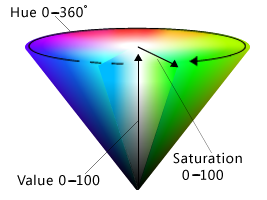
\includegraphics[width=0.3\textwidth]{images/hsv.png}
\caption{The HSV model, a cone having three parameters: Hue, Saturation and Value.}
\label{hsv}
\end{figure}

For filtering a certain colour in a image we define the ranges of the colour that has to be filtered. Every pixel is checked whether it is within this range, if so the pixel in the result image is set to 1 otherwise to 0. This result image is a binary image, where the colours in range of the colour are set to white. Colour filtering reduces the amount of noise caused by other colours in the image.

% TODO: REWRITTEN
\subsubsection{Canny Edge Detector}
The Canny Edge Detector \cite{Canny1986} is an edge detection operator that uses a multi-stage algorithm to detect edges. The aim of Canny was to develop a edge detector algorithm that is optimal for the following aspects:
\begin{description}
\item[Good detection] by marking the most real edges in the image.
\item[Good localization] by marking the edges as close to the real edge.
\item[Minimal response] by only marking edges once.
\end{description}
Calculus of variations, a mathematical technique that finds the optimal function, was applied to fulfil these requirements. The algorithm consists of the following four stages in order to reach edge detection: Noise reduction, finding the intensity gradient, non-maximum suppression and hysteresis threshold. These stages will be explained in the next sections.\\

\noindent\textbf{Noise reduction}\\
Noise reduction is applied to raw image data as the edge detector is sensitive to noise. Noise reduction can be realized by using convolution with a suitable kernel. The Canny edge detector uses a Gaussian kernel as this is a suitable kernel. This phenomenon is called Gaussian Smoothing (see appendix \ref{gaussiansmoothing}) and filters out the small distortions so these are not detected by the edge detector. Gaussian Smoothing results into a smoothed image.\\

\noindent\textbf{Finding the intensity gradient}\\
After the noise reduction the directional change in intensity, the gradient, is calculated for every pixel  in the image. The gradient of every pixel in the image may point in a variety of directions. Therefore, the Canny Edge Detector uses four filters to detect horizontal, vertical and diagonal edges in the smoothed image. In order to find the gradient in the image the algorithm uses a edge detection operator, which takes the first derivative of the image that results in the gradient in horizontal direction $Gx$ and vertical direction $Gy$. There are a variety of edge detection operators and the one applied in this thesis is the Sobel operator. The Sobel operator convolves (see appendix \ref{gaussiansmoothing}) two $3\times3$ kernels with the image $A$ to find the horizontal $Gx$ and vertical  $Gy$ derivative, which is described in equation \ref{sobel}.
\begin{equation}
\label{sobel}
Gx =
\begin{bmatrix}
-1 & 0 & 1\\
-2 & 0 & 2\\
-1 & 0 & 1
\end{bmatrix}
* A\ \ \ \ \ 
Gy =
\begin{bmatrix}
-1 & -2 & -1\\
0 & 0 & 0\\
1 & 2 & 1
\end{bmatrix}
* A
\end{equation}
From the derivatives the gradient $G$ and direction $\Theta$ can be determined, this is illustrated in equation \ref{gradient}.
\begin{equation}
\label{gradient}
G = \sqrt{G_x^2  + G_y^2}\ \ \ \ \ 
\Theta = \arctan(\frac{G_x}{G_y})
\end{equation}
The directional angle is rounded to one of the four angles representing vertical, horizontal or the two diagonals in order to reduce computational costs of the algorithm.\\ 

\noindent\textbf{Non-maximum suppression}\\
Non-maximum suppression is the process of scanning a image along the image gradient direction. The pixels that are not part of the local maxima are set to zero. This suppresses all image information that is not part of the local maxima. Given the image gradient and direction estimates the algorithm seeks for the local maxima in the gradient direction by looping over the pixels of the image. For example, if the rounded gradient angle of the pixel is zero degrees, the pixel pointing downwards, the gradient magnitude is compared to the gradient magnitude of its left and right neighbour. If the gradient magnitude of the pixel is greater than its neighbours it will be considered a possible edge. Non-maximum suppression removes pixels that are not considered to be part of an edge. Therefore, only thin lines, candidate edges, will remain. This stage results in a binary image containing a set of possible edge points.\\

\noindent\textbf{Hysteresis thresholding}\\
The large intensity gradients are more probable to correlate to edges than small intensity gradients. For this reason, it is impossible to specify a threshold to determine whether a certain gradient is a edge or not. Therefore, the Canny Edge Detector applies another technique, namely, thresholding with hysteresis. In thresholding with hysteresis a upper and lower threshold is defined. The algorithm makes the assumption that important edges should be along continuous curves in the image, which allows the algorithm to follow a faint section of a given line and to ignore a few noisy pixels that have large gradients. Thresholding with hysteresis selects edges on the following basis:
\begin{itemize}
\item All candidates above the upper threshold will be selected as edges
\item All candidates below the lower will be refused as edges
\item All candidates between the upper and lower threshold will only be selected if it is connected to a pixel that is above the upper threshold.
\end{itemize}
This is the final of the Canny Edge Detector and results into a boolean image representing the edges in the image.

\begin{figure}

[Insert image]

\caption{Left: original image. Middle: smoothed image. Right: Edge image produced by the Canny Edge Detector}
\label{canny}
\end{figure}


\subsection{Motion Detector Algorithm}
Motion detection is a tool in Computer Vision that is applied to detect whether an object has changed its position relative to its surroundings or the surroundings have changed relative to an object. Motion can be detected by mechanical and electronic methods. Motion can be detected by various sensors such as: sound, ultrasonic and opacity. This thesis focuses on opacity as the platform has only a limited sensor suite (see chapter \ref{platform}). 

\subsubsection{Motion detector}
To be written.
\subsection{Probabilistic Hough Line Transform}
To be written.
\subsection{Tracking}
To be written.
\subsection{Navigation}
To be written.
\newpage
\section{Related Work}
One of the essential requirements of a autonomous robot is the ability of navigation in the real world environment. One of the main problems in navigation is that no sensor is reliable enough to function in every environment. The most commonly used sensor currently for outside navigation is the GPS. GPS receiver requires to receive data signals from four different satellites to be able to localize itself. Additionally, the measurements can contain errors due to the influences (ie. signal reflection) of the surrounding environment. Due to these restrictions GPS cannot operate inside buildings and in several outdoor urban environments. Therefore, to navigate through these environments other sensors and navigation techniques have to be investigated.\\

More to be written.
Comments:
Ik mis o.a. Bills et al ICRA 2011 (following corridors with an AR.Drone) en de artikelen die naar Bills verwijzen.
Een andere mogelijkheid is het onderzoek gerelateerd aan UUV die pipelines volgen.
Ik wil in ieder geval hier een opsomming van de artikelen die je wil gaan bespreken.

\newpage
\section{Platform: Parrot AR.Drone}
\label{platform}
One of the basic steps for the development and testing of intelligent applications in robotics is to find an applicable robot platform for the defined problem. A common choice is to use a quadcopter, which is  mainly designed to be a Unmanned Aerial Vehicle (UAV). The small size and manoeuvrability allows both indoor and outdoor flights. Moreover, quadcopters have a simple design due to the fact that they do not require mechanical connections to vary the pitch angle of rotor blade.

As a result of technological developments in aerospace engineering of UAV's, a small quadcopter with on-board stabilization can be purchased conveniently. Because of this, research regarding this platform is moving towards more intelligent applications, which demand information of the surrounding environment. The specific platform selected for the experiments in this research is the Parrot AR.Drone quadcopter. The advantages of this platform are its on-board stabilization, lightweight and the affordable price of the platform. The AR.Drone is carrying a front and bottom camera that provide live video streaming through the data link. Additionally, it has an ultrasound sensor and an inertial measurement unit that measures the pitch, roll, yaw and accelerations of the platform. The platform is controlled via WiFi, which allows the user to send commands and receive data of the platform.

In this chapter, the AR.Drone platform is described. The operational part of te platform is discussed, the hardware the platform contains is described and the software development kit is briefly described.

\subsection{Quadcopter}
A quadcopter consists of four rotors that are attached to a main frame, which commonly has a cross-shaped form (see figure \ref{quadcopter}). Every rotor produces thrust $T$ and torque $\tau$ over the center of rotation, whereas it also produces drag force $D_b$ in the opposite direction of flight. Thrust $T$ is the force that is generated by increasing and decreasing acceleration the mass in one direction. The acceleration of the mass will result in a force of equal magnitude but in the opposite direction of the platform. Torque $\tau$ is the force that rotates an object around its axis. Drag $D_b$ is the force that is in opposite direction to the motion of the aircraft through air. This force is inclined on the velocity of the quadcopter and de-acceleration will take place if insufficient thrust is generated. The rotors together should generate sufficient thrust to stay airborne during flights.

\begin{figure}[!ht]
	\centering
	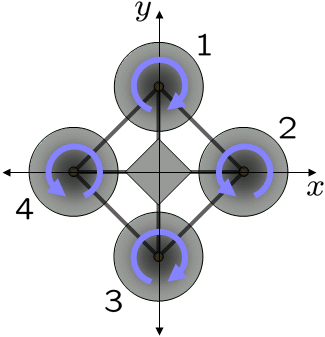
\includegraphics[width=0.25\textwidth]{images/quadcopter.png}
	\caption{Diagram of the reaction torgues on each motor of the quadcopter, due to the rotors. Rotors one and three are spinning clockwise, whereas rotor two and four spin counter-clockwise, causing opposing force for control}
	\label{quadcopter}
\end{figure}

In order to fly the quadcopter relies on differences in thrust and torque. Pitch, roll and yaw (see figure \ref{plane}) is the naming of flight dynamics to indicate the rotation angles in three dimension of the center mass of the quadcopter. The opposing rotor pairs (pair 1, 3 and pair 2, 4) turn in the same direction. One of the pairs is turning clockwise, while the other pair turns counter-clockwise. This causes the platform to have no angular acceleration, when all rotor pairs have the same angular acceleration. Alternating the angular speed of the rotor pairs will cause angular acceleration about the yaw.

\begin{figure}[!ht]
	\centering
	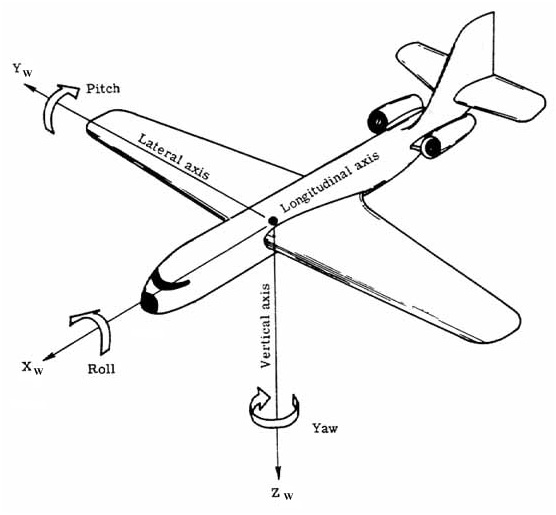
\includegraphics[width=0.5\textwidth]{images/plane.jpg}
	\caption{Diagram of pitch, roll and yaw rotations on an aerial vehicle}
	\label{plane}
\end{figure}

Vertical movements are accomplished by changing the thrust from each rotor alike, which is causing the resulting thrust to change and the differential torque to remain zero. Moreover, when the thrust is kept constant the vertical velocity remains the same. Horizontal movements are caused by changing the pitch and roll angle. Angular accelerations over the pitch and roll angles can be generated independently. Each pair of opposing rotors controls either pitch or roll rotation of the platform. A torque balance is kept for yaw stability during differential torque over the roll and pitch by increasing the speed of one rotor, while decreasing the speed of the opposing rotor.

\subsection{Hardware}
The AR.Drone is a remote-controlled quadcopter developed by the french company Parrot SA for consumer use. The main frame is made of carbon fibre and high resistance plastic. The AR.Drone has an indoor and outdoor hull, which is used for protection of the system. The rotors are powered by motors, whom are connected to a lithium battery allowing the system to fly ten minutes.

\subsubsection{AR.Drone 1.0}
The AR.Drone has an on-board computer running a custom Linux operating system. A mini-USB connector is included on the system for software maintenance and additional external sensors (e.g. GPS sensor). The integrated wireless card provides network access for external devices that control the vehicle. The software of the AR.Drone is available for all platforms, however, the most supported software is written for iOS devices (ie. Apple iPhone). Nevertheless, it is possible to create controlling applications for the Windows and Linux platforms. Furthermore, the AR.Drone has a sensor suite containing an six degrees of freedom Inertial Measurement Unit (IMU), a bottom camera and a ultrasound altimeter used for automatic stabilization. The IMU consists of a three axis accelerometer, a two axis roll and pitch gyrometer and a single axis yaw gyrometer. The IMU reports on the system its velocity, orientation and gravitational forces. The ultrasound altimeter measure the altitude of the system and in combination with the bottom camera it calculates the optical flow of the system. All the above sensors contribute to the on-board stabilization module of the quadcopter, which allows the quadcopter to hover in one place. Additionally, the system carries a frontal camera to provide the operator with visual feedback.

The horizontal camera has approximately 75$^{\circ}$ x 60$^{\circ}$ field of view and provides 640 x 480 pixel color images. The bottom camera provides color images with 176 x 144 pixels and its field of view is approximately 45$^{\circ}$ x 35$^{\circ}$ \cite{Krajnik2011}.

\subsubsection{AR.Drone 2.0}
Recently, Parrot brought a new platform on the market, the AR.Drone 2.0. This new platform has a similar configuration as its predecessor, however, most of the components have been improved. The new on-board technology gives better stabilization and more precise sensor measurement comparing to their previous platform. The AR.Drone two carries a horizontal camera with a resolution of 1280 x 720 pixels and the vertical camera a resolution of 320 x 240 pixels. These improvements aid intelligent vision-based applications as more detailed images give more information about the environment.

\subsection{Software Development Kit}
Parrot created a open source Software Development Kit (SDK) providing developers the opportunity to create intelligent applications for their platform. The SDK comes with source code, multiplatform examples and documentation. The SDK does not provide software that is embedded on the AR.Drone itself. The SDK implements the following three channels of communications with the platform:
\begin{enumerate}
\item Configuration and control of the platform.
\item Status of the platform (ie. altitude, attitude and speed).
\item Video stream.
\end{enumerate}
These four channels of communication can be used for designing intelligent applications for the AR.Drone.

\section{Framework: AR.Drone SLAM}
\label{framework}
To be written.
\section{Experiments}
To be written.
\section{Results}
To be written.
\section{Discussion}
To be written.
\section{Conclusion}
To be written.
\newpage
\begin{appendices}
\section{Source code}
All the source code is available at the GitHub repository:\\ \url{https://github.com/camielv/ThesisVerschoor}.\\
The recorded datasets are available here:\\
\url{https://github.com/camielv/ThesisVerschoor/Datasets}\\
A research log can be found here:\\
\url{http://camielv.nl/thesis}

\newpage
\section{Gaussian Smoothing}
\label{gaussiansmoothing}
% TODO: REWRITTEN
This chapter provides a explanation for Gaussian Smoothing. The convolution technique is discussed first and then the Gaussian kernel of convolution is explained.\\

\noindent\textbf{Convolution}\\
Convolution is a mathematical way to combine two functions. The mathematical definition of convolution for the two scalar functions $f(x)$ and $g(x)$ is:
\begin{equation*}
h(x) = \int_{-\infty}^\infty f(u)g(x - u)du
\end{equation*}

The integral expresses the amount of overlap of function $g(x)$
due the shift over the other function $f(x)$. This causes one function to blend with the other. The convolution operator contains the following algebraic properties: commutativity, associativity and distributivity. Convolution is commonly applied in computer vision in order to detect edges in a image. In figure \ref{gaussianblur} a example of a convolution with the Gaussian Kernel is illustrated.
\begin{figure}[!ht]
\centering
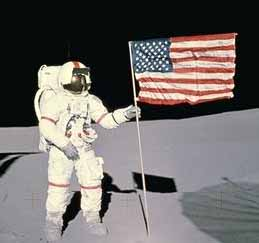
\includegraphics[width=0.22\textwidth]{images/gaussianblur_before.jpg}
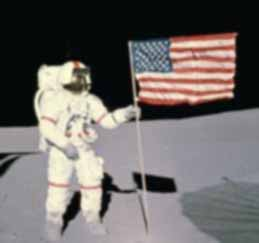
\includegraphics[width=0.22\textwidth]{images/gaussianblur_after1.jpg}
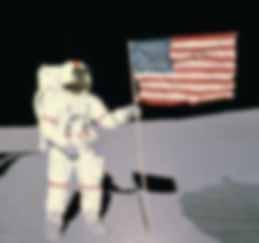
\includegraphics[width=0.22\textwidth]{images/gaussianblur_after2.jpg}
\caption[Gaussian Blur]{Left: original. Middle and right: Gaussian Blur of 1.2 and 2.5 pixels. Images by \href{http://www.websupergoo.com/helpie/}{WebSupergoo}}.
\label{gaussianblur}
\end{figure}

\noindent\textbf{Gaussian Kernel}\\
The most suitable kernel for an optimal convolution is the Gaussian function due to the smoothing, derivatives and separability. The Gaussian function has the best smoothing properties as it has existing derivatives to any order at every point. Due to this every function can be smoothed as the derivative is always non-zero. In image processing the intensity is smooth smoothed intensity of a image this can be done by convolving the original image with the derivative of the Gaussian function. Gaussian Smoothing is the result of blurring an image by a Gaussian Function. Smoothing is applied to reduce noise and detail in the image. Gaussian smoothing is a well know technique mostly used in computer vision algorithms as a pre-processing technique in order to enhance image structures at different scales. Gaussian Smoothing is the same as convolving the image with a Gaussian function. The 2D Gaussian smoothing function is represented by the following equation:
\begin{equation*}
G(x,y) = \frac{1}{2\pi\sigma^2}e^{\frac{x^2 + y^2}{2\sigma^2}}
\end{equation*}

\section{Ascending Technologies Pelican}
\label{pelican}
To be written.
\end{appendices}

\newpage

% BIBLIOGRAPHY
\section{Bibliography}
\renewcommand{\section}[2]{}
\bibliographystyle{apalike}
\bibliography{references}
\end{document}
